\subsection{Warped Extra Dimensions}\label{sec:wed}
In the Warped Extra Dimensions (WED) model~\cite{Randall:1999ee,Carvalho:2014lsg}, a five-dimensional geometry is proposed where a small spatial dimension is added to the traditional 4D spacetime. This theory alleviates the hierarchy problem and introduces two new \textit{gravity particles}: a spin-0 boson called the Radion which we denote \XZero, and a spin-2 boson called the Graviton which we denote \XTwo. Two theoretical scenarios are described in Ref.~\cite{Carvalho:2014lsg}, one where the SM particles are not allowed to propagate along the extra dimension and another where they are allowed, and these scenarios are referred to as the RS1 and Bulk scenarios respectively.

The decay channels and branching fractions for the Radion and Graviton are shown in \cref{fig:WED_BF}. In the Bulk scenario, the branching fraction to two SM Higgs bosons is about 30\% and about 10\% for the Radion and Graviton respectively for masses above 300\GeV. There are higher branching fractions to other decay channels such as \WW but more sensitive searches can be achieved with \HH if the right Higgs boson decay channels are chosen. One of the most competitive \HH decay channels is $b\bar{b}\gamma\gamma$ which has lower backgrounds and better mass resolution compared to $\PX \to \PW\PW$. 

Even better constraints can be achieved by performing searches with additional Higgs boson decay channels and then combining these searches, and this motivates the \XHH search in the $\gamma\gamma\tau\tau$ final state presented in \cref{chap:dihiggs}. In the RS1 scenario, the $\XTwo \to \PH\PH$ decay channel has a significantly lower branching fraction of around $\sim0.5\%$. Therefore, the search in \cref{chap:dihiggs} only considers the Bulk scenario. Production cross sections for the Radion and Graviton at $\sqrt{s}=13\TeV$ in the Bulk scenario are shown in \cref{fig:WED_xs} for particular values of $kl$, $\Lambda_R$ and $\tilde{k}$ which are free parameters of the theory and described in Ref.~\cite{Carvalho:2014lsg}. The dominant production mode for both the Radion and Graviton is gluon-gluon fusion.

\begin{figure}
  \centering
  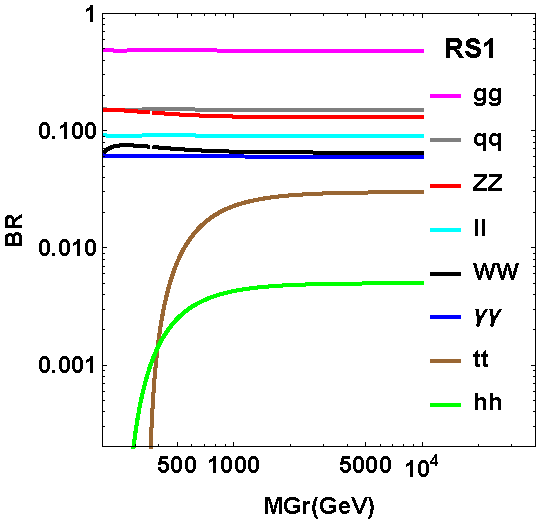
\includegraphics[width=0.49\textwidth]{Figures/Theory/WED/RSGravitonBRanal.pdf}
  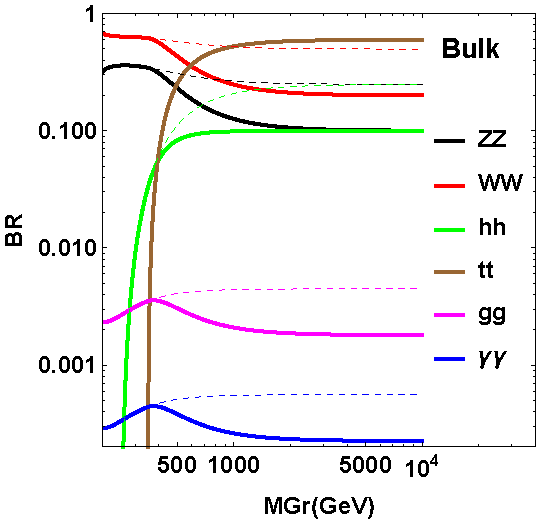
\includegraphics[width=0.49\textwidth]{Figures/Theory/WED/BulkGravitonBRanalWitTop.pdf}
  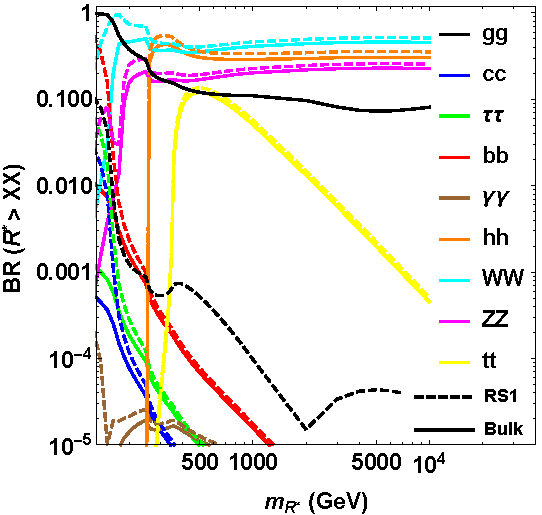
\includegraphics[width=0.49\textwidth]{Figures/Theory/WED/BR_eHDecay.pdf}
  \caption[Graviton and Radion Branching Fractions]{Branching fractions for the Graviton (top) and Radion (bottom) as functions of the particle masses. The RS1 and Bulk scenarios for the Graviton are shown in the top-left and top-right respectively whereas for the Radion, they are shown on the same plot and are differentiated by dashed and solid lines respectively. Figures are taken from Ref.~\cite{Carvalho:2014lsg}.}\label{fig:WED_BF}
\end{figure}

\begin{figure}
  \centering
  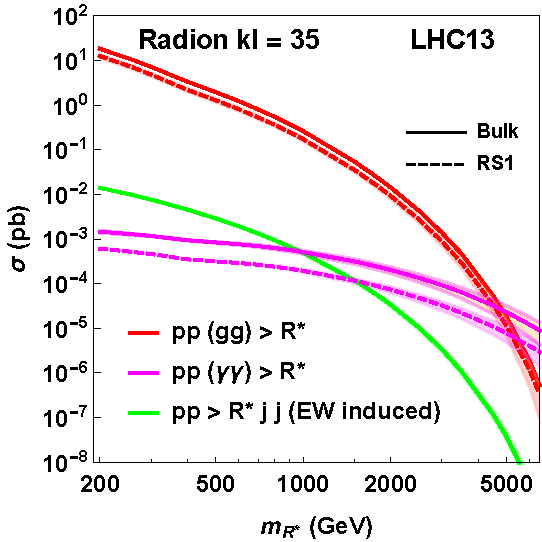
\includegraphics[width=0.48\textwidth]{Figures/Theory/WED/CX_RS_radion_13tev.pdf}
  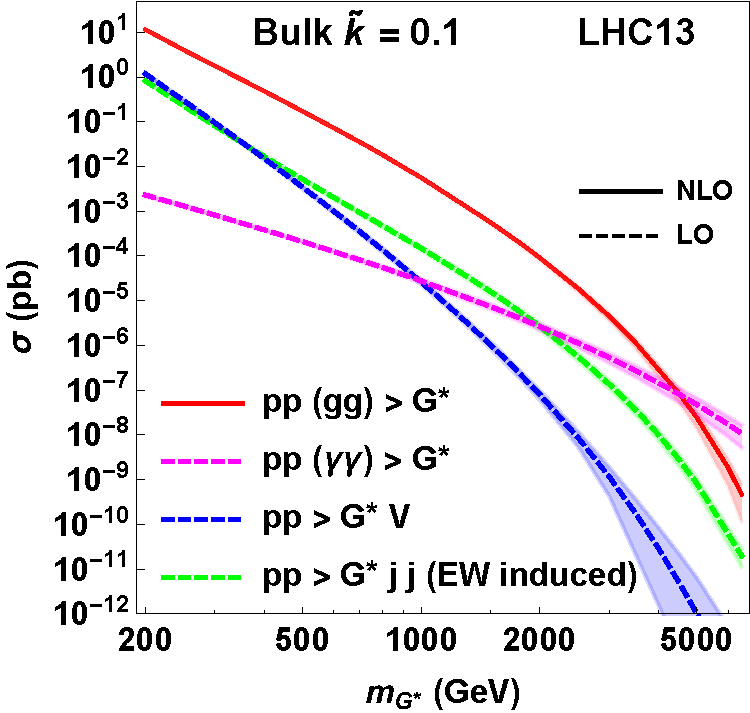
\includegraphics[width=0.49\textwidth]{Figures/Theory/WED/CX_bulk_13tev.pdf}
  \caption[Graviton and Radion Production Cross Sections]{Production cross sections at the LHC with $\sqrt{s}=13\TeV$ for the Radion ($R^*$) on the left, and the Graviton ($G^*$) on the right, shown as functions of the resonance masses. The Radion cross sections are shown for $kl=35$ and $\Lambda_R=3$\TeV and the Graviton cross sections are shown for $\tilde{k}=0.1$. Figures are taken from Ref.~\cite{Carvalho:2014lsg}.}\label{fig:WED_xs}
\end{figure}

